\documentclass{article}
%\documentstyle[11pt,handout,psfig]{article}

\usepackage{fullpage,amssymb,amsmath,epsf}
\usepackage[12pt]{extsizes}

%These give really tight margins:
%\setlength{\topmargin}{-0.3in}
%\setlength{\textheight}{8.10in}
%\setlength{\textwidth}{5.8in}
%\setlength{\baselineskip}{0.1875in}
%\addtolength{\leftmargin}{-2.775in}
%\setlength{\footskip}{0.45in}
%\setlength{\oddsidemargin}{0.5in}
%\setlength{\evensidemargin}{0.5in}
%%\setlength{\headsep}{0pt}
%%\setlength{\headheight}{0pt}

%\setlength{\topmargin}{-0.5in}
\setlength{\textheight}{8in}
%\setlength{\textwidth}{5.0in}
%\setlength{\baselineskip}{0.1875in}
%\addtolength{\leftmargin}{-2.775in}
%\setlength{\footskip}{0.45in}
%\setlength{\oddsidemargin}{0.5in}
%\setlength{\evensidemargin}{0.5in}
%%\setlength{\headsep}{0pt}
%%\setlength{\headheight}{0pt}


\markright{CS229 Winter 2003}
\pagestyle{myheadings}

\newcommand{\newsec}{\section}
\newcommand{\denselist}{\itemsep 0pt\partopsep 0pt}
\newcommand{\bitem}{\begin{itemize}\denselist}
\newcommand{\eitem}{\end{itemize}}
\newcommand{\benum}{\begin{enumerate}\denselist}
\newcommand{\eenum}{\end{enumerate}}

\newcommand{\fig}[1]{\private{\begin{center}
{\Large\bf ({#1})}
\end{center}}}

\newcommand{\cpsf}[1]{{\centerline{\psfig{#1}}}}
\newcommand{\mytitle}[1]{\centerline{\LARGE\bf #1}}

\newcommand{\myw}{{\bf w}}

\newcommand{\mypar}[1]{\vspace{1ex}\noindent{\bf {#1}}}

\def\thmcolon{\hspace{-.85em} {\bf :} }

\newtheorem{THEOREM}{Theorem}[section]
\newenvironment{theorem}{\begin{THEOREM} \thmcolon }%
                        {\end{THEOREM}}
\newtheorem{LEMMA}[THEOREM]{Lemma}
\newenvironment{lemma}{\begin{LEMMA} \thmcolon }%
                      {\end{LEMMA}}
\newtheorem{COROLLARY}[THEOREM]{Corollary}
\newenvironment{corollary}{\begin{COROLLARY} \thmcolon }%
                          {\end{COROLLARY}}
\newtheorem{PROPOSITION}[THEOREM]{Proposition}
\newenvironment{proposition}{\begin{PROPOSITION} \thmcolon }%
                            {\end{PROPOSITION}}
\newtheorem{DEFINITION}[THEOREM]{Definition}
\newenvironment{definition}{\begin{DEFINITION} \thmcolon \rm}%
                            {\end{DEFINITION}}
\newtheorem{CLAIM}[THEOREM]{Claim}
\newenvironment{claim}{\begin{CLAIM} \thmcolon \rm}%
                            {\end{CLAIM}}
\newtheorem{EXAMPLE}[THEOREM]{Example}
\newenvironment{example}{\begin{EXAMPLE} \thmcolon \rm}%
                            {\end{EXAMPLE}}
\newtheorem{REMARK}[THEOREM]{Remark}
\newenvironment{remark}{\begin{REMARK} \thmcolon \rm}%
                            {\end{REMARK}}
%\newenvironment{proof}{\noindent {\bf Proof:} \hspace{.677e\nexp}}%
%                      {}

%theorem
\newcommand{\thm}{\begin{theore\nexp}}
%lemma
\newcommand{\lem}{\begin{lemma}}
%proposition
\newcommand{\pro}{\begin{propositio\di}}
%definition
\newcommand{\dfn}{\begin{definitio\di}}
%remark
\newcommand{\rem}{\begin{remark}}
%example
\newcommand{\xam}{\begin{example}}
%corollary
\newcommand{\cor}{\begin{corollary}}
%proof
\newcommand{\prf}{\noindent{\bf Proof:} }
%end theorem
\newcommand{\ethm}{\end{theore\nexp}}
%end lemma
\newcommand{\elem}{\end{lemma}}
%end proposition
\newcommand{\epro}{\end{propositio\di}}
%end definition
\newcommand{\edfn}{\bbox\end{definitio\di}}
%end remark
\newcommand{\erem}{\bbox\end{remark}}
%end example
\newcommand{\exam}{\bbox\end{example}}
%end corollary
\newcommand{\ecor}{\end{corollary}}
%end proof
\newcommand{\eprf}{\bbox\vspace{0.1i\di}}
%begin equation
\newcommand{\beqn}{\begin{equatio\di}}
%end equation
\newcommand{\eeqn}{\end{equatio\di}}

%\newcommand{\eqref}[1]{Eq.~\ref{#1}}

\newcommand{\KB}{\mbox{\it KB\/}}
\newcommand{\infers}{\vdash}
\newcommand{\sat}{\models}
\newcommand{\bbox}{\vrule height7pt width4pt depth1pt}

\newcommand{\act}[1]{\stackrel{{#1}}{\rightarrow}}
\newcommand{\at}[1]{^{(#1)}}

\newcommand{\argmax}{{\rm argmax}}

\newcommand{\rimp}{\Rightarrow}
\newcommand{\dimp}{\Leftrightarrow}

\newcommand{\bX}{\mbox{\boldmath $X$}}
\newcommand{\bY}{\mbox{\boldmath $Y$}}
\newcommand{\bZ}{\mbox{\boldmath $Z$}}
\newcommand{\bU}{\mbox{\boldmath $U$}}
\newcommand{\bE}{\mbox{\boldmath $E$}}
\newcommand{\bx}{\mbox{\boldmath $x$}}
\newcommand{\be}{\mbox{\boldmath $e$}}
\newcommand{\by}{\mbox{\boldmath $y$}}
\newcommand{\bz}{\mbox{\boldmath $z$}}
\newcommand{\bu}{\mbox{\boldmath $u$}}
\newcommand{\bd}{\mbox{\boldmath $d$}}
\newcommand{\smbx}{\mbox{\boldmath $\scriptstyle x$}}
\newcommand{\smbd}{\mbox{\boldmath $\scriptstyle d$}}
\newcommand{\smby}{\mbox{\boldmath $\scriptstyle y$}}
\newcommand{\smbe}{\mbox{\boldmath $\scriptstyle e$}}

\newcommand{\Parents}{\mbox{\it Parents\/}}
\newcommand{\B}{{\cal B}}
\newcommand{\calH}{{\cal H}}

\newcommand{\word}[1]{\mbox{\it #1\/}}
\newcommand{\Action}{\word{Actio\di}}
\newcommand{\Proposition}{\word{Propositio\di}}
\newcommand{\true}{\word{true}}
\newcommand{\false}{\word{false}}
\newcommand{\Pre}{\word{Pre}}
\newcommand{\Add}{\word{Add}}
\newcommand{\Del}{\word{Del}}
\newcommand{\Result}{\word{Result}}
\newcommand{\Regress}{\word{Regress}}
\newcommand{\Maintain}{\word{Maintai\di}}

\newcommand{\bor}{\bigvee}
\newcommand{\invert}[1]{{#1}^{-1}}

\newcommand{\commentout}[1]{}

\newcommand{\bmu}{\mbox{\boldmath $\mu$}}
\newcommand{\btheta}{\mbox{\boldmath $\theta$}}
\newcommand{\IR}{\mbox{$I\!\!R$}}

\newcommand{\tval}[1]{{#1}^{1}}
\newcommand{\fval}[1]{{#1}^{0}}

\newcommand{\tr}{{\rm tr}}
\newcommand{\vecy}{{\vec{y}}}
\renewcommand{\Re}{{\mathbb R}}

\def\twofigbox#1#2{%
\noindent\begin{minipage}{\textwidth}%
\epsfxsize=0.35\maxfigwidth
\noindent \epsffile{#1}\hfill
\epsfxsize=0.35\maxfigwidth
\epsffile{#2}\\
\makebox[0.35\textwidth]{(a)}\hfill\makebox[0.35\textwidth]{(b)}%
\end{minipage}}

\def\twofigboxcd#1#2{%
\noindent\begin{minipage}{\textwidth}%
\epsfxsize=0.35\maxfigwidth
\noindent \epsffile{#1}\hfill
\epsfxsize=0.35\maxfigwidth
\epsffile{#2}\\
\makebox[0.35\textwidth]{(c)}\hfill\makebox[0.35\textwidth]{(d)}%
\end{minipage}}

\def\twofigboxnolabel#1#2{%
\begin{minipage}{\textwidth}%
\epsfxsize=0.35\maxfigwidth
\noindent \epsffile{#1}\hfill
\epsfxsize=0.35\maxfigwidth
\epsffile{#2}\\
%\makebox[0.48\textwidth]{(a)}\hfill\makebox[0.48\textwidth]{(b)}%
\end{minipage}
}

\def\twofigboxnolabelFive#1#2{%
\begin{minipage}{\textwidth}%
\hbox to 0.5in{}\epsfxsize=0.35\maxfigwidth
\noindent \epsffile{#1}\hfill
\epsfxsize=0.35\maxfigwidth
\epsffile{#2}\hbox to 0.5in{}\\
%\makebox[0.48\textwidth]{(a)}\hfill\makebox[0.48\textwidth]{(b)}%
\end{minipage}
}

\def\threefigbox#1#2#3{%
\noindent\begin{minipage}{\textwidth}%
\epsfxsize=0.33\maxfigwidth
\noindent \epsffile{#1}\hfill
\epsfxsize=0.33\maxfigwidth
\noindent \epsffile{#2}\hfill 
\epsfxsize=0.33\maxfigwidth
\epsffile{#3}\\
\makebox[0.31\textwidth]{{\scriptsize (a)}}\hfill%
\makebox[0.31\textwidth]{{\scriptsize (b)}}\hfill
\makebox[0.31\textwidth]{{\scriptsize (c)}}%
\smallskip
\end{minipage}}

\def\threefigboxnolabel#1#2#3{%
\noindent\begin{minipage}{\textwidth}%
\epsfxsize=0.33\maxfigwidth
\noindent \epsffile{#1}\hfill
\epsfxsize=0.33\maxfigwidth
\noindent \epsffile{#2}\hfill 
\epsfxsize=0.33\maxfigwidth
\epsffile{#3}\\
%\makebox[0.31\textwidth]{{\scriptsize (a)}}\hfill%
%\makebox[0.31\textwidth]{{\scriptsize (b)}}\hfill
%\makebox[0.31\textwidth]{{\scriptsize (c)}}%
%\smallskip
\end{minipage}}

\newlength{\maxfigwidth}
\setlength{\maxfigwidth}{\textwidth}
%\def\captionsize {\footnotesize}
\def\captionsize {}

\newcommand{\xsi}{{x^{(i)}}}
\newcommand{\xsd}{{x^{(d)}}}
\newcommand{\xsj}{{x^{(j)}}}
\newcommand{\ysi}{{y^{(i)}}}
\newcommand{\ysj}{{y^{(j)}}}
\newcommand{\gsi}{{\gamma^{(i)}}}
\newcommand{\wsi}{{w^{(i)}}}
\newcommand{\esi}{{\epsilon^{(i)}}}
\newcommand{\calN}{{\cal N}}
\newcommand{\calX}{{\cal X}}
\newcommand{\calY}{{\cal Y}}
\newcommand{\calL}{{\cal L}}
\newcommand{\calP}{{\cal P}}
\newcommand{\calD}{{\cal D}}
\newcommand{\ytil}{{\tilde{y}}}

\newcommand{\Ber}{{\rm Bernoulli}}
\newcommand{\E}{{\rm E}}

\newcommand{\pstar}{{p^{\ast}}}
\newcommand{\bstar}{{b^{\ast}}}
\newcommand{\dstar}{{d^{\ast}}}
\newcommand{\wstar}{{w^{\ast}}}
\newcommand{\alphastar}{\alpha^{\ast}}
\newcommand{\alphastari}{{\alpha_i^{\ast}}}
\newcommand{\betastar}{{\beta^{\ast}}}
\newcommand{\tol}{{\textit tol}}
\newcommand{\phihat}{\hat\phi}
\newcommand{\ehat}{\hat\varepsilon}
\newcommand{\hhat}{\hat{h}}
\newcommand{\hstar}{h^\ast}
\newcommand{\VC}{{\rm VC}}

\newcommand{\hwb}{{h_{w,b}}}

\usepackage{graphicx}

%\renewcommand{\epsffile}[1]{
%	\includegraphics[width=\epsfxsize]{#1}
%}

\newcommand{\di}{{d}}
\newcommand{\nexp}{{n}}
\newcommand{\vcd}{{\textbf{D}}}

\begin{document}
\title{XCS229i Lecture Notes}
\author{Andrew Ng}
\date{}
\maketitle


\setcounter{part}{10}
\part{Principal components analysis}

%In this set of notes, we continue our discussion of unsupervised learning.

In our discussion of factor analysis, we gave a way to model data $x \in \Re^\di$ as ``approximately'' lying in some $k$-dimension subspace, where $k \ll \di$. Specifically, we imagined that each point $\xsi$ was created by first generating some $\zsi$ lying in the $k$-dimension affine space $\{\Lambda z+\mu; z \in \Re^k\}$, and then adding $\Psi$-covariance noise. Factor analysis is based on a probabilistic model, and parameter estimation used the iterative EM algorithm.

In this set of notes, we will develop a method, Principal Components Analysis (PCA), that also tries to identify the subspace in which the data approximately lies. However, PCA will do so more directly, and will require only an eigenvector calculation (easily done with the {\tt eig} function in Matlab), and does not need to resort to EM.

Suppose we are given a dataset $\{\xsi; i=1, \ldots, \nexp\}$ of attributes of $\nexp$ different types of automobiles, such as their maximum speed, turn radius, and so on.
%and on which we wish to do some learning.
Let $\xsi \in \Re^\di$ for each $i$ ($\di \ll \nexp$). But unknown to us, two different attributes---some $x_i$ and $x_j$---respectively give a car's maximum speed measured in miles per hour, and the maximum speed measured in kilometers per hour. These two attributes are therefore almost linearly dependent, up to only small differences introduced by rounding off to the nearest mph or kph. Thus, the data really lies approximately on an $n-1$ dimensional subspace. How can we automatically detect, and perhaps remove,
this redundancy?

For a less contrived example, consider a dataset resulting from a survey of pilots for radio-controlled helicopters, where $x^{(i)}_1$ is a measure of the piloting skill of pilot $i$, and $x^{(i)}_2$ captures how much he/she enjoys flying. Because RC helicopters are very difficult to fly, only the most committed students, ones that truly enjoy flying, become good pilots. So, the two attributes $x_1$ and $x_2$ are strongly correlated. Indeed, we might posit that that the data actually likes along some diagonal axis (the $u_1$ direction) capturing the intrinsic piloting ``karma'' of a person, with only a small amount of noise lying off this axis. (See figure.) How can we automatically compute this $u_1$ direction?

\begin{center}
% eps library outdated
% \epsfxsize=3in
% \epsffile{heliPilot.eps}
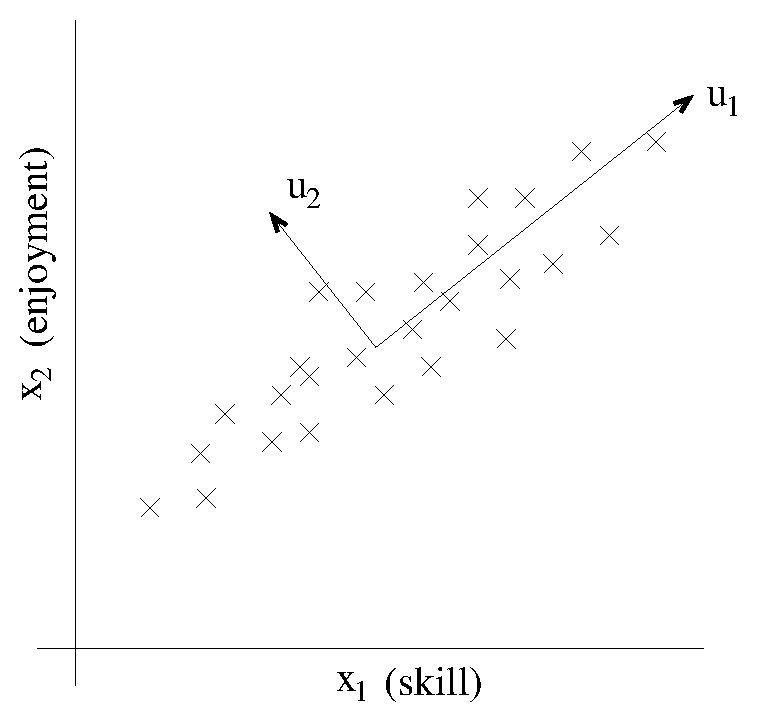
\includegraphics[scale=0.5]{heliPilot.eps}
\end{center}

We will shortly develop the PCA algorithm. But prior to running PCA per se, typically we first preprocess the data by normalizing each feature to have mean 0 and variance 1. We do this by subtracting the mean and dividing by the empirical standard deviation:
$$
x^{(i)}_j \leftarrow \frac{x^{(i)}_j - \mu_j}{\sigma_j}
$$
where $\mu_j = \frac{1}{\nexp} \sum_{i=1}^\nexp x^{(i)}_j$ and $\sigma_j^2 = \frac{1}{\nexp} \sum_{i=1}^\nexp (x^{(i)}_j - \mu_j)^2$ are the mean variance of feature $j$, respectively.

Subtracting $\mu_j$ zeros out the mean and may be omitted for data known to have zero mean (for instance, time series corresponding to speech or other acoustic signals). Dividing by the standard deviation $\sigma_j$ rescales each coordinate to have unit variance, which ensures that different attributes are all treated on the same ``scale.'' For instance, if $x_1$ was cars' maximum speed in mph (taking values in the high tens or low hundreds) and $x_2$ were the number of seats (taking values around 2-4), then this renormalization rescales the different attributes to make them more comparable. This rescaling may be omitted if we had a priori knowledge that the different attributes are all on the same scale. One example of this is if each data point represented a grayscale image, and each $x^{(i)}_j$ took a value in $\{0, 1, \ldots, 255\}$ corresponding to the intensity value of pixel $j$ in image $i$.

Now, having normalized our data, how do we compute the ``major axis of variation'' $u$---that is, the direction on which the data approximately lies? One way is to pose this problem as finding the unit vector $u$ so that when the data is projected onto the direction corresponding to $u$, the variance of the projected data is maximized. Intuitively, the data starts off with some amount of variance/information in it. We would like to choose a direction $u$ so that if we were to approximate the data as lying in the direction/subspace corresponding to $u$, as much as possible of this variance is still retained.

Consider the following dataset, on which we have already carried out the normalization steps:
\begin{center}
% eps library outdated
% \epsfxsize=3in
% \epsffile{rawdata.eps}
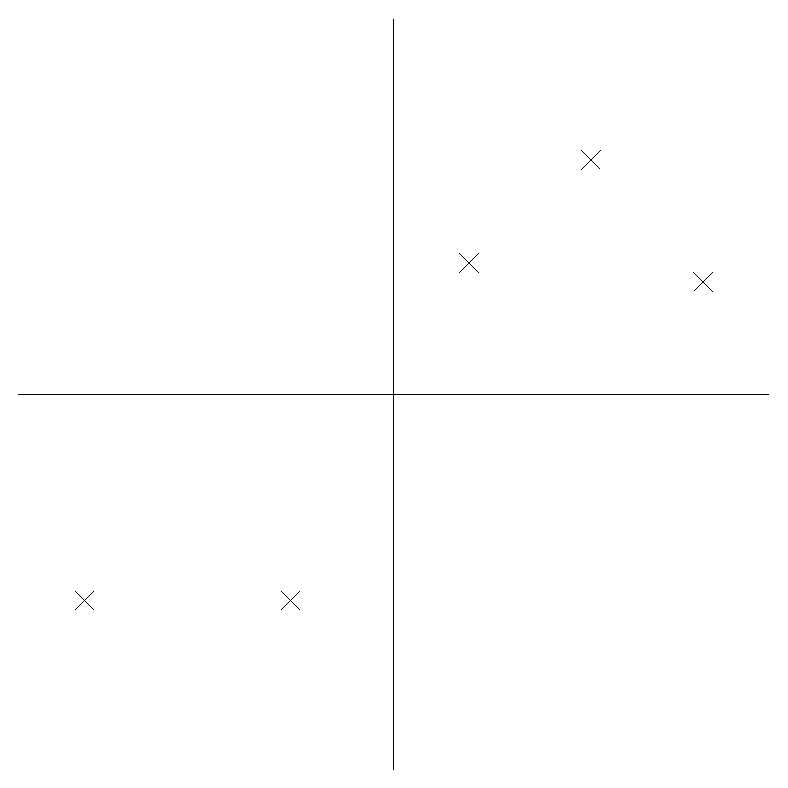
\includegraphics[scale=0.5]{rawdata.eps}
\end{center}

Now, suppose we pick $u$ to correspond the the direction shown in the figure below. The circles denote the projections of the original data onto this line.
\begin{center}
% eps library outdated
% \epsfxsize=3in
% \epsffile{proj1.eps}
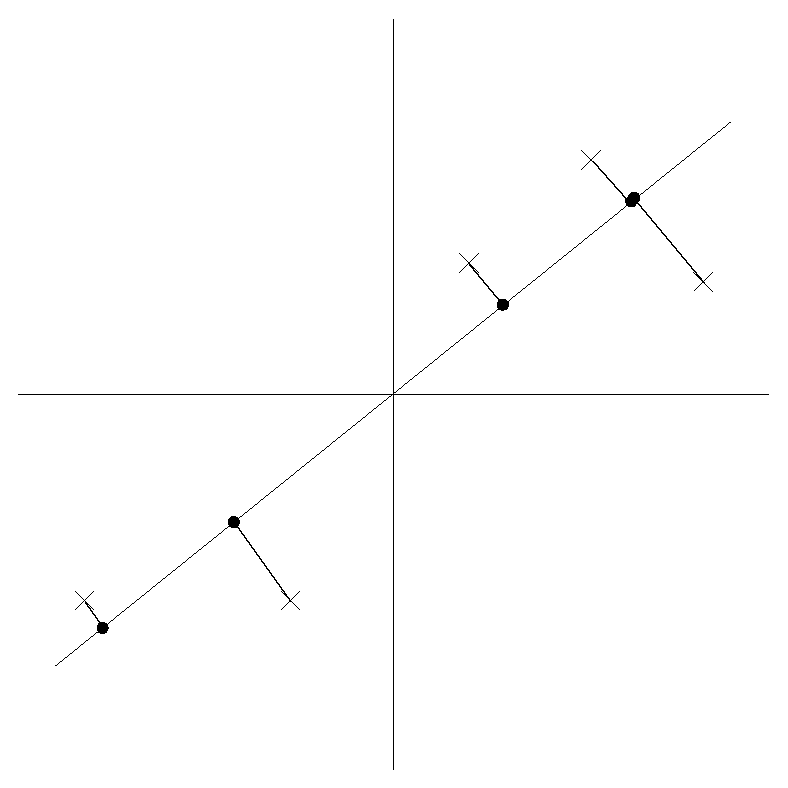
\includegraphics[scale=0.5]{proj1.eps}
\end{center}

We see that the projected data still has a fairly large variance, and the points tend to be far from zero. In contrast, suppose had instead picked the following direction:

\begin{center}
% eps library outdated
% \epsfxsize=3in
% \epsffile{proj2.eps}
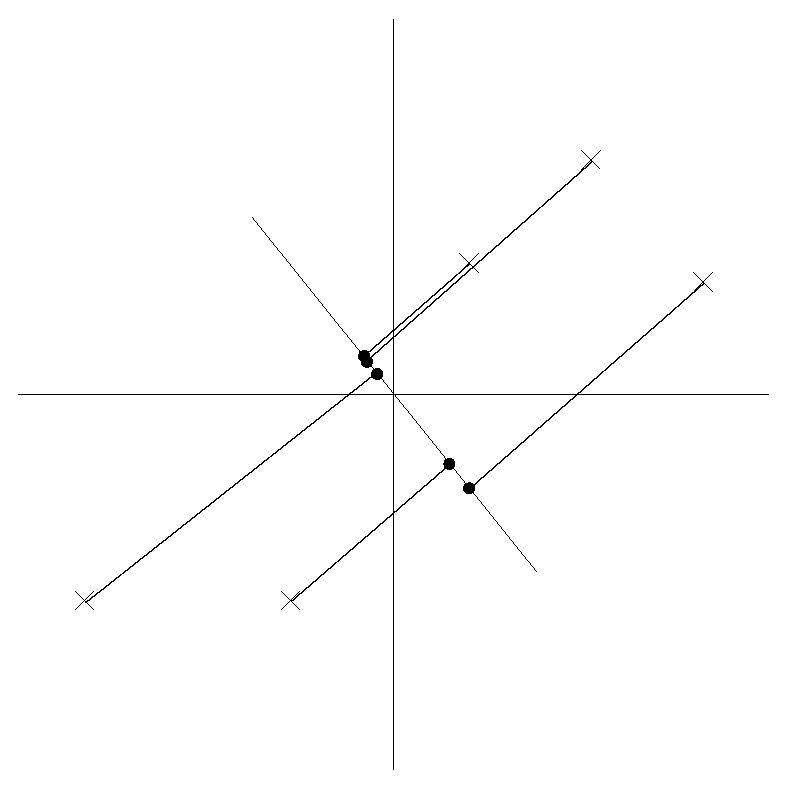
\includegraphics[scale=0.5]{proj2.eps}
\end{center}

Here, the projections have a significantly smaller variance, and are much closer to the origin.

We would like to automatically select the direction $u$ corresponding to the first of the two figures shown above. To formalize this, note that given a unit vector $u$ and a point $x$, the length of the projection of $x$ onto $u$ is given by $x^Tu$. I.e., if $\xsi$ is a point in our dataset (one of the crosses in the plot), then its projection onto $u$ (the corresponding circle in the figure) is distance $x^Tu$ from the origin. Hence, to maximize the variance of the projections, we would like to choose a unit-length $u$ so as to maximize:
\begin{align*}
\frac{1}{\nexp} \sum_{i=1}^\nexp (\xsi^T u)^2
&= \frac{1}{\nexp} \sum_{i=1}^\nexp u^T\xsi \xsi ^T u \\
&= u^T \left( \frac{1}{\nexp} \sum_{i=1}^\nexp \xsi \xsi^T \right) u.
\end{align*}
We easily recognize that the maximizing this subject to $\|u\|_2=1$ gives the
principal eigenvector of $\Sigma = \frac{1}{\nexp} \sum_{i=1}^\nexp \xsi \xsi^T$, which
is just the empirical covariance matrix of the data (assuming it has zero mean).\footnote{If you
haven't seen this before, try using the method of Lagrange multipliers to maximize
$u^T\Sigma u$ subject to that $u^Tu=1$. You should be able to show that $\Sigma u = \lambda u$,
for some $\lambda$, which implies $u$ is an eigenvector of $\Sigma$, with eigenvalue $\lambda$.}

To summarize, we have found that if we wish to find a 1-dimensional subspace with with to approximate the data, we should choose $u$ to be the principal eigenvector of $\Sigma$. More generally, if we wish to project our data into a $k$-dimensional subspace ($k < \di$), we should choose $u_1, \ldots, u_k$ to be the top $k$ eigenvectors of $\Sigma$. The $u_i$'s now form a new, orthogonal basis for the data.\footnote{Because $\Sigma$ is symmetric, the $u_i$'s will (or always can be chosen to be) orthogonal to each other.}

Then, to represent $\xsi$ in this basis, we need only compute the corresponding vector
\[
\ysi = \begin{bmatrix}
    u_1^T \xsi \\
    u_2^T \xsi \\
    \vdots \\
    u_k^T \xsi
\end{bmatrix}
\in \Re^k.
\]
Thus, whereas $\xsi \in \Re^\di$, the vector $\ysi$ now gives a lower, $k$-dimensional, approximation/representation for $\xsi$. PCA is therefore also referred to as a {\bf dimensionality reduction} algorithm. The vectors $u_1, \ldots, u_k$ are called the first $k$ {\bf principal components} of the data.

\medskip
\noindent
{\bf Remark.} Although we have shown it formally only for the case of $k=1$, using well-known properties of eigenvectors it is straightforward to show that of all possible orthogonal bases $u_1, \ldots, u_k$, the one that we have chosen maximizes $\sum_i \|\ysi\|_2^2$. Thus, our choice of a basis preserves as much variability as possible in the original data.
\medskip

In problem set 4, you will see that PCA can also be derived by picking the basis that minimizes the approximation error arising from projecting the data onto the $k$-dimensional subspace spanned by them.

PCA has many applications; we will close our discussion with a few examples. First, compression---representing $\xsi$'s with lower dimension $\ysi$'s---is an obvious application. If we reduce high dimensional data to $k=2$ or $3$ dimensions, then we can also plot the $\ysi$'s to visualize the data. For instance, if we were to reduce our automobiles data to 2 dimensions, then we can plot it (one point in our plot would correspond to one car type, say) to see what cars are similar to each other and what groups of cars may cluster together.

Another standard application is to preprocess a dataset to reduce its dimension before running a supervised learning learning algorithm with the $\xsi$'s as inputs. Apart from computational benefits, reducing the data's dimension can also reduce the complexity of the hypothesis class considered and help avoid overfitting (e.g., linear classifiers over lower dimensional input spaces will have smaller VC dimension).

Lastly, as in our RC pilot example, we can also view PCA as a noise reduction algorithm. In our example it, estimates the intrinsic ``piloting karma'' from the noisy measures of piloting skill and enjoyment. In class, we also saw the application of this idea to face images, resulting in {\bf eigenfaces} method. Here, each point $\xsi \in \Re^{100\times 100}$ was a 10000 dimensional vector, with each coordinate corresponding to a pixel intensity value in a 100x100 image of a face. Using PCA, we represent each image $\xsi$ with a much lower-dimensional $\ysi$. In doing so, we hope that the principal components we found retain the interesting, systematic variations between faces that capture what a person really looks like, but not the ``noise'' in the images introduced by minor lighting variations, slightly different imaging conditions, and so on. We then measure distances between faces $i$ and $j$ by working in the reduced dimension, and computing $\|\ysi - \ysj\|_2$. This resulted in a surprisingly good face-matching and retrieval algorithm.

%\begin{center}
%\epsfxsize=3in
%\epsffile{foo.eps}
%\end{center}

\end{document}
